% Created 2023-08-21 Mon 20:30
% Intended LaTeX compiler: pdflatex
\documentclass[10pt, a4paper, twoside, headinclude,footinclude, BCOR5mm]{scrartcl}
\usepackage[utf8]{inputenc}
\usepackage[T1]{fontenc}
\usepackage{graphicx}
\usepackage{longtable}
\usepackage{wrapfig}
\usepackage{rotating}
\usepackage[normalem]{ulem}
\usepackage{amsmath}
\usepackage{amssymb}
\usepackage{capt-of}
\usepackage{hyperref}
\usepackage[nochapters, beramono, eulermath, pdfspacing, dottedtoc]{classicthesis}
\usepackage{arsclassica}
\usepackage[T1]{fontenc}
\usepackage[utf8]{inputenc}
\usepackage{amsmath,amssymb,amsthm}
\usepackage{enumitem}
\usepackage{parskip}
\usepackage{tcolorbox}
\publishers{\normalsize{University of Twente, Faculty of Engineering Technology \\ Mechanics of Solids, Surfaces and Systems, Chair of Production Technology}}
\author{Wouter Grouve}
\date{}
\title{1D Heat Conduction\\\medskip
\large FE formulation}
\hypersetup{
 pdfauthor={Wouter Grouve},
 pdftitle={1D Heat Conduction},
 pdfkeywords={Conduction, FE, Derivation},
 pdfsubject={},
 pdfcreator={Emacs 29.1 (Org mode 9.6.6)}, 
 pdflang={English}}
\begin{document}

\maketitle


\section{Introduction}
\label{sec:org36ffbe6}


\section{Derivation}
\label{sec:orgfedd426}

\subsection{Governing partial differential equation and weak form}
\label{sec:org0f53657}

In the case of 1D heat conduction, the governing partial equation reads:
\begin{equation}
  \label{eq:pde}
  \rho c_\text{p}\frac{\partial T}{\partial z} -
  k_{\text{z}}\frac{\partial^2 T}{\partial z^2} -
  \dot{Q} = 0
\end{equation}
with \(T\) the temperature, \(\rho c_{\text{p}}\) the volumetric heat capacity, \(k_{\text{z}}\) the thermal conductivity, and \(\dot{Q}\) an internal  source or sink, e.g. due to a phase transformation. The partial differential equation is subject to boundary conditions at the two ends of the domain, which can be of the Dirichlet type:
\begin{equation*}
  T(0,t) = T_\text{left}(t), \qquad T(L,t) = T_\text{right}(t),
\end{equation*}
or of the Neumann type:
\begin{equation*}
  -k_{\text{z}}\frac{\partial T}{\partial z}\Biggr|_{z=0} = q_\text{left}(t), \qquad
  -k_{\text{z}}\frac{\partial T}{\partial z}\Biggr|_{z=L} = q_{\text{right}}(t),
\end{equation*}
with \(T_\text{left}\) and \(T_\text{right}\) an imposed temperature and \(q_\text{left}\) and \(q_\text{right}\) an imposed heat flux density. The latter could be either directly imposed \(\hat{q}\), for example as a result of laser heating, or be the result of convection:
\begin{equation*}
  q = h(T_{\infty}-T),
\end{equation*}
in which \(h\) and \(T_{\infty}\) are the heat transfer coefficient and the far field temperature, or the result of thermal radiation:
\begin{equation*}
  q = \epsilon\sigma(T_{\infty}^4-T^4),
\end{equation*}
where \(\epsilon\) is the surface emissivity and \(\sigma\) is Stefan's constant.

We can approximate the solution \(T(z,t)\) of the partial differential equation using the weighted residual method:
\begin{equation}
  \label{eq:weighted_residual}
  \int_L w\left(
  \rho c_\text{p} \frac{\partial T}{\partial t} -
  k_\text{z} \frac{\partial^2 T}{\partial z^2} -
  \dot{Q} \right) \text{d}z = 0,
\end{equation}
with \(w\) a weighting function.


\subsection{Discretization in space}
\label{sec:org702fc48}

The domain in \(N\) is now split up in smaller elements, as is indicated in Figure \ref{fig:orgc4dbac9} which shows an element \((e)\) of length \(\ell\) that is bounded by the nodes \(i\) and \(j\). The weighted residual (Equation \ref{eq:weighted_residual}) can now be rewritten as:
\begin{equation}
  \label{eq:weighted_residual_sum}
  \sum_{e=1}^N
  \int_\ell w\left(
    \rho c_\text{p}\frac{\partial T}{\partial t} -
    k_\text{z}\frac{\partial^2 T}{\partial z^2} -
    \dot{Q} \right) \text{d}z = 0.
\end{equation}
We will now make sure that the weighted residual vanishes for each element. Further, we get rid of the second derivative with respect to \(z\) in the second term using integration by parts:
\begin{equation*}
  \int_\ell w \rho c_\text{p}\frac{\partial T}{\partial t} \text{d}z +
  \int_\ell
  \frac{\text{d}w}{\text{d}z}k_\text{z}\frac{\partial T}{\partial z}\text{d}z -
  wk_\text{z}\frac{\partial T}{\partial z}\Biggr|_{z_i}^{z_j} -
  \int_\ell w \dot{Q} \text{d}z = 0,
\end{equation*}
with \(z_i\) and \(z_j\) the element end points. Realizing that the third term represents the flux (\(q = -k \partial T / \partial z\)), the equation can be rewritten as:
\begin{equation}
  \label{eq:weighted_residual_el}
  \int_\ell w \rho c_\text{p}\frac{\partial T}{\partial t} \text{d}z +
  \int_\ell
  \frac{\text{d}w}{\text{d}z}k_\text{z}\frac{\partial T}{\partial z}\text{d}z
  = \int_\ell w \dot{Q} \text{d}z -
  w q \Biggr|_{z_i}^{z_j}.
\end{equation}

\begin{figure}[htbp]
\centering
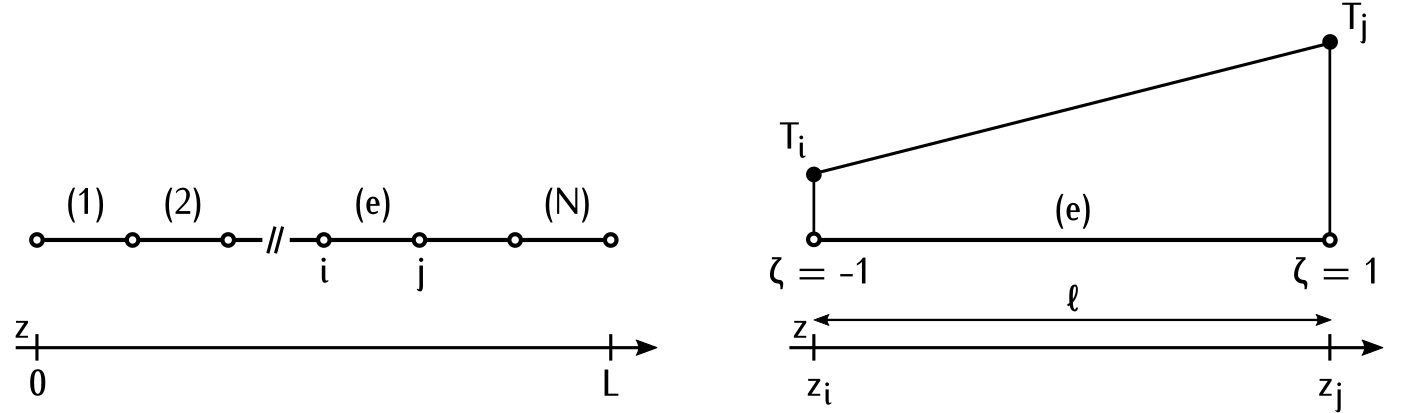
\includegraphics[width=.9\linewidth]{./fig/elements_sf.png}
\caption{\label{fig:orgc4dbac9}Left: Elements in 1D domain. Right: Definition of local coordinate system and linear interpolation of temperature.}
\end{figure}

\subsubsection{Linear shape functions}
\label{sec:orgb421675}

The temperature inside an element is approximated as a linear interpolation between the bounding node temperatures as:
\begin{equation}
\label{eq:T_approx}
  T(\zeta) = N_i(\zeta)T_i + N_j(\zeta)T_j,
\end{equation}
with \(\zeta\) a local coordinate, as is illustrated in Figure \ref{fig:orgc4dbac9}, defined as:
\begin{equation*}
  \zeta(z) = 2\frac{z - (z_j - z_i)/2}{\ell},
\end{equation*}
while the two shape functions are:
\begin{equation}
  \label{eq:shape_functions}
  N_i(\zeta) = \frac{1-\zeta}{2} \quad\text{and}\quad
  N_j(\zeta) = \frac{1+\zeta}{2}.
\end{equation}
The spatial derivative of the temperature with respect to \(z\) can now be calculated as:
\begin{equation*}
  \frac{\partial T}{\partial z} =
  \frac{\partial T}{\partial \zeta}\frac{\partial \zeta}{\partial z},
\end{equation*}
with:
\begin{equation*}
  \frac{\partial \zeta}{\partial z} = \frac{2}{\ell}
  \quad\text{and}\quad
  \frac{\partial T}{\partial \zeta} = \frac{T_2 - T_1}{2},
\end{equation*}
such that:
\begin{equation}
  \label{eq:dTdz}
  \frac{\partial T}{\partial z} = \frac{T_2 - T_1}{\ell},
\end{equation}
which also intuitively makes sense of course. Further, noting that the shape functions do not depend on time, we can rewrite the time derivative as:
\begin{equation}
  \label{eq:dTdt}
  \frac{\partial T}{\partial t} =
  N_i(\zeta)\frac{\partial T_i}{\partial t} +
  N_j(\zeta)\frac{\partial T_j}{\partial t}.
\end{equation}

Following the Galerkin method, we choose our weighting function \(w\) to be our shape functions. The equation for the weighted residual for an element (Equation \ref{eq:weighted_residual_el}) can now be rewritten as:
\begin{equation}
  \label{eq:galerkin}
  \int_\ell N_k \rho c_\text{p}\frac{\partial T}{\partial t} \text{d}z +
  \int_\ell
  \frac{\text{d}N_k}{\text{d}z}k_\text{z}\frac{\partial T}{\partial z}\text{d}z  =
  \int_\ell N_k \dot{Q} \text{d}z - N_k q \Biggr|_{z_i}^{z_j}
  \quad\text{for: } k = 1,2.
\end{equation}
with \(N_i\) and \(N_j\) the two shape functions as defined in Equation \ref{eq:shape_functions}.

\begin{tcolorbox}[colback=gray!5,colframe=gray!40!black,title=Matrix-vector notation]
Before evaluating the integrals, we first rewrite the expressions from the previous section into a matrix-vector form. Starting with Equation \ref{eq:T_approx}, which can be written as:
\begin{equation*}
  T(\zeta) = \bold{N}\bold{T},
\end{equation*}
in which:
\begin{equation*}
\bold{N} = [N_i(\zeta), N_j(\zeta)] \quad\text{and}\quad
\bold{T} = \begin{Bmatrix} T_i \\ T_j \end{Bmatrix} \,
\end{equation*}
The spatial derivative of the temperature (Equation \ref{eq:dTdz}) yields:
\begin{equation*}
  \frac{\partial T}{\partial z} =
  \frac{\partial}{\partial z}\left(\bold{N}\bold{T}\right) =
  \bold{B}\bold{T},
\end{equation*}
with:
\begin{equation*}
  \bold{B} = \frac{\partial \bold{N}}{\partial z} =
  \left[\frac{\partial N_i}{\partial z}, \frac{\partial N_j}{\partial z}\right] =
  \left[-\frac{1}{\ell}, \frac{1}{\ell}\right],
\end{equation*}
while the time-derivative of the temperature can be rewritten as:
\begin{equation*}
  \frac{\partial T}{\partial t} =
  \bold{N}\bold{\dot{T}}.
\end{equation*}
Further, for convenience, we will write our weighting functions as:
\begin{equation*}
  w = \bold{N}^T = \begin{Bmatrix} N_i \\ N_j \end{Bmatrix}.
\end{equation*}
\end{tcolorbox}

We can now evaluate the integrals, starting with the first term:
\begin{equation*}
  \int_\ell w \rho c_\text{p}\frac{\partial T}{\partial t} \text{d}z =
  \rho c_\text{p}\int_\ell \bold{N}^T \bold{N} \text{d}z \; \bold{\dot{T}}.
\end{equation*}
We can rewrite this integral in terms of \(\zeta\), by making use of the derivative of \(\zeta\) with respect to \(z\):
\begin{equation*}
  \frac{\text{d}\zeta}{\text{d}z} = \frac{2}{\ell} \quad\rightarrow\quad
  \text{d}z = \frac{\ell}{2}\text{d}\zeta,
\end{equation*}
such that:
\begin{equation}
\label{eq:C}
  \rho c_\text{p} \int_\ell \bold{N}^T \bold{N}\text{d}z \;\bold{\dot{T}} =
  \frac{\ell\rho c_\text{p}}{2}\int_{-1}^{1} \bold{N}^T \bold{N} \text{d}\zeta \; \bold{\dot{T}} =
  \bold{C}\bold{\dot{T}},
\end{equation}
with:
\begin{equation*}
  \bold{C} = \frac{\ell\rho c_\text{p}}{2}\int_{-1}^{1} \bold{N}^T\bold{N} \text{d}\zeta =
  \frac{\ell\rho c_\text{p}}{6}\left[\begin{matrix} 2 & 1\\
                                               1 & 2\end{matrix}\right].
\end{equation*}

In the same manner, the second term yields:
\begin{equation}
\label{eq:K}
  \int_\ell \frac{\text{d}N_k}{\text{d}z}k_\text{z}\frac{\partial T}{\partial z}\text{d}z =
  \frac{\ell k_\text{z}}{2} \int_{-1}^{1} \bold{B}^T \bold{B} \text{d}\zeta \;\bold{T} = \bold{K} \bold{T},
\end{equation}
with:
\begin{equation*}
  \bold{K} = \frac{\ell k_\text{z}}{2} \int_{-1}^{1} \bold{B}^T \bold{B} \text{d}\zeta =
  \frac{k_\text{z}}{\ell}\left[\begin{matrix} 1 & -1\\
                                              -1 & 1\end{matrix}\right].
\end{equation*}

The first term on the right hand side yields:
\begin{equation*}
  \int_\ell \bold{N}^T \dot{Q} \text{d}z =
  \frac{\ell}{2} \int_{-1}^{1} \bold{N} \text{d}\zeta \; \dot{Q} = \frac{ \dot{Q} \ell}{2} \begin{Bmatrix} 1 \\ 1 \end{Bmatrix},
\end{equation*}
with \(\dot{Q}\) the heat source term for the element between nodes \(i\) and \(j\). The second term with the heat flux \(q\) on the boundary is first expanded to include both a direct heat flux \(\hat{q}\) and a flux due to convection:
\begin{equation*}
  q = \hat{q} + h(T_{\infty}-T),
\end{equation*}
which yields:
\begin{equation*}
  N_k q \Biggr|_{z_i}^{z_j} = N_k \hat{q} \Biggr|_{z_i}^{z_j} +
                             N_k h (T_{\infty}-T) \Biggr|_{z_i}^{z_j}.
\end{equation*}
The term with the direct heat flux \(\hat{q}\) is evaluated as:
\begin{equation*}
  N_k \hat{q} \Biggr|_{z_i}^{z_j} =
     \begin{Bmatrix} N_i(z_j)q_j - N_i(z_i) \hat{q}_i \\
                     N_j(z_j)q_j - N_j(z_i) \hat{q}_i \end{Bmatrix} =
     \begin{Bmatrix} - \hat{q}_i \\
                       \hat{q}_j \end{Bmatrix},
\end{equation*}
with \(\hat{q}_k\) the heat flux on the \(k\)-th node. The convective term can be accounted for using a stiffness matrix for convection:
\begin{equation}
\label{eq:H}
  N_k h T \Biggr|_{z_i}^{z_j} = \bold{H} \bold{T} \quad{with:}\quad
      \bold{H} = h\left[\begin{matrix} N_i N_i & N_i N_j \\
                                       N_j N_i & N_j N_j \end{matrix}\right],
\end{equation}
and an additional term in the force vector:
\begin{equation*}
  N_k h T_{\infty} \Biggr|_{z_i}^{z_j} =
     h\begin{Bmatrix} - T_{\infty,i} \\
                        T_{\infty,j} \end{Bmatrix}.
\end{equation*}
As an example for the stiffness matrix \(\bold{H}\), in case of a convective boundary condition at the j-th node, where \(N_i = 0\), this term would evaluate as:
\begin{equation*}
  \bold{H} = \left[\begin{matrix} N_i N_i & N_i N_j \\
                                  N_j N_i & N_j N_j \end{matrix}\right] =
             \left[\begin{matrix} 0 & 0 \\
                                  0 & 1 \end{matrix}\right],
\end{equation*}
which intuitively makes sense. The force vector is now combined as:
\begin{equation}
\label{eq:f}
\bold{f} = \int_\ell N_k \dot{Q} \text{d}z - N_k q \Biggr|_{z_i}^{z_j} -          N_k h T_{\infty} \Biggr|_{z_i}^{z_j} =
           \frac{\dot{Q}\ell}{2}\begin{Bmatrix} 1 \\ 1\end{Bmatrix} +
           \begin{Bmatrix}  \hat{q}_i \\
                            -\hat{q}_j \end{Bmatrix} +
           h\begin{Bmatrix}  T_{\infty,i} \\
                             -T_{\infty,j} \end{Bmatrix}.
\end{equation}

The final element equation can now be assembled from by subsituting Equations \ref{eq:C}, \ref{eq:K}, \ref{eq:H} and \ref{eq:f} in Equation \ref{eq:galerkin}:
\begin{equation*}
\bold{C}\bold{\dot{T}} + (\bold{K} + \bold{H})\bold{T} = \bold{f}.
\end{equation*}

With the local damping and stiffness matrices determined for each element, we can assemble  the global matrices using the element locations in the global system.

\subsubsection{Quadratic shape functions}
\label{sec:org9310202}

bla

\subsection{Temporal discretization}
\label{sec:org7facc3b}

The final step is to integrate the equation with time. For this purpose, we will descretize the temporal variable will using the so-called \(\Theta\)-method:
\begin{equation}
\label{eq:theta}
  \bold{C} \frac{\bold{T}_{\text{n}+1} - \bold{T}_\text{n}}{\Delta t} +
  (1-\Theta)(\bold{K}+\bold{H}) \bold{T}_{\text{n}} +
  \Theta(\bold{K}+\bold{H}) \bold{T}_{\text{n}+1}
  =
  (1-\Theta)\bold{f}_{\text{n}} + \Theta\bold{f}_{\text{n}+1},
\end{equation}
where \(\Theta \in [0, 1]\). Common values of \(\Theta\) are:
\begin{eqnarray*}
  \Theta =& 0,   &\qquad\text{(Explit Euler)}\\
  \Theta =& 1/2, &\qquad\text{(Crank Nicolson)}\\
  \Theta =& 1,   &\qquad\text{(Implicit Euler)}.
\end{eqnarray*}
Equation \ref{eq:theta} can be rearranged as:
\begin{equation*}
  \Bigl( \bold{C} + \Delta t\Theta(\bold{K}+\bold{H})
  \Bigr) \bold{T}_{\text{n}+1} =
  \Bigl(
  \bold{C} - \Delta t(1-\Theta)(\bold{K}+\bold{H})
  \Bigr) \bold{T}_{\text{n}} +
  \Delta t(1-\Theta)\bold{f}_{\text{n}} +
  \Delta t\Theta\bold{f}_{\text{n}+1}.
\end{equation*}


\section{Validation}
\label{sec:org032e414}

\subsection{Step temperature at boundary}
\label{sec:org394f742}

Consider a domain of length \(L\) with a uniform initial temperature \(T_0\). For \(t>0\) the temperature at one end is raised to a value of \(T_{\text{end}}\), while the other end is kept at the initial temperature:
\begin{eqnarray*}
  T(x, 0) =& T_0\\
  T(0, t) =& T_0\\
  T(L, t) =& T_{\text{end}}
\end{eqnarray*}
In case the initial temperature equals 0.0 \(^{\circ}\)C , the analytical solution\footnote{The Mathematics of Diffusion, Crank, 1975} yields:
\begin{equation}
T(x) = \frac{T_{\text{end}}x}{L} + \frac{2}{\pi}
       \sum_{N=1}^{\infty} \frac{T_{\text{end}} \cos N\pi}{N}
       \sin\left(\frac{N\pi x}{L}\right)
       \exp\left(-\alpha N^2 \pi^2 t / L^2 \right),
\end{equation}
with \(\alpha = k/\rho c_{\text{p}}\) the thermal diffusivity. The left graph in Figure \ref{fig:step_compare} shows the temperature distribution at different times for a domain with properties as listed in Table \ref{tbl:prop}. The right graphs shows the corresponding finite element solution for 10 linear elements of equal length. Good comparison is obtained between the numerical and analytical solution. The code for this comparison is available in the Python file \texttt{step\_change.py}.

\begin{figure}
\centering
\begin{minipage}{.5\textwidth}
  \centering
  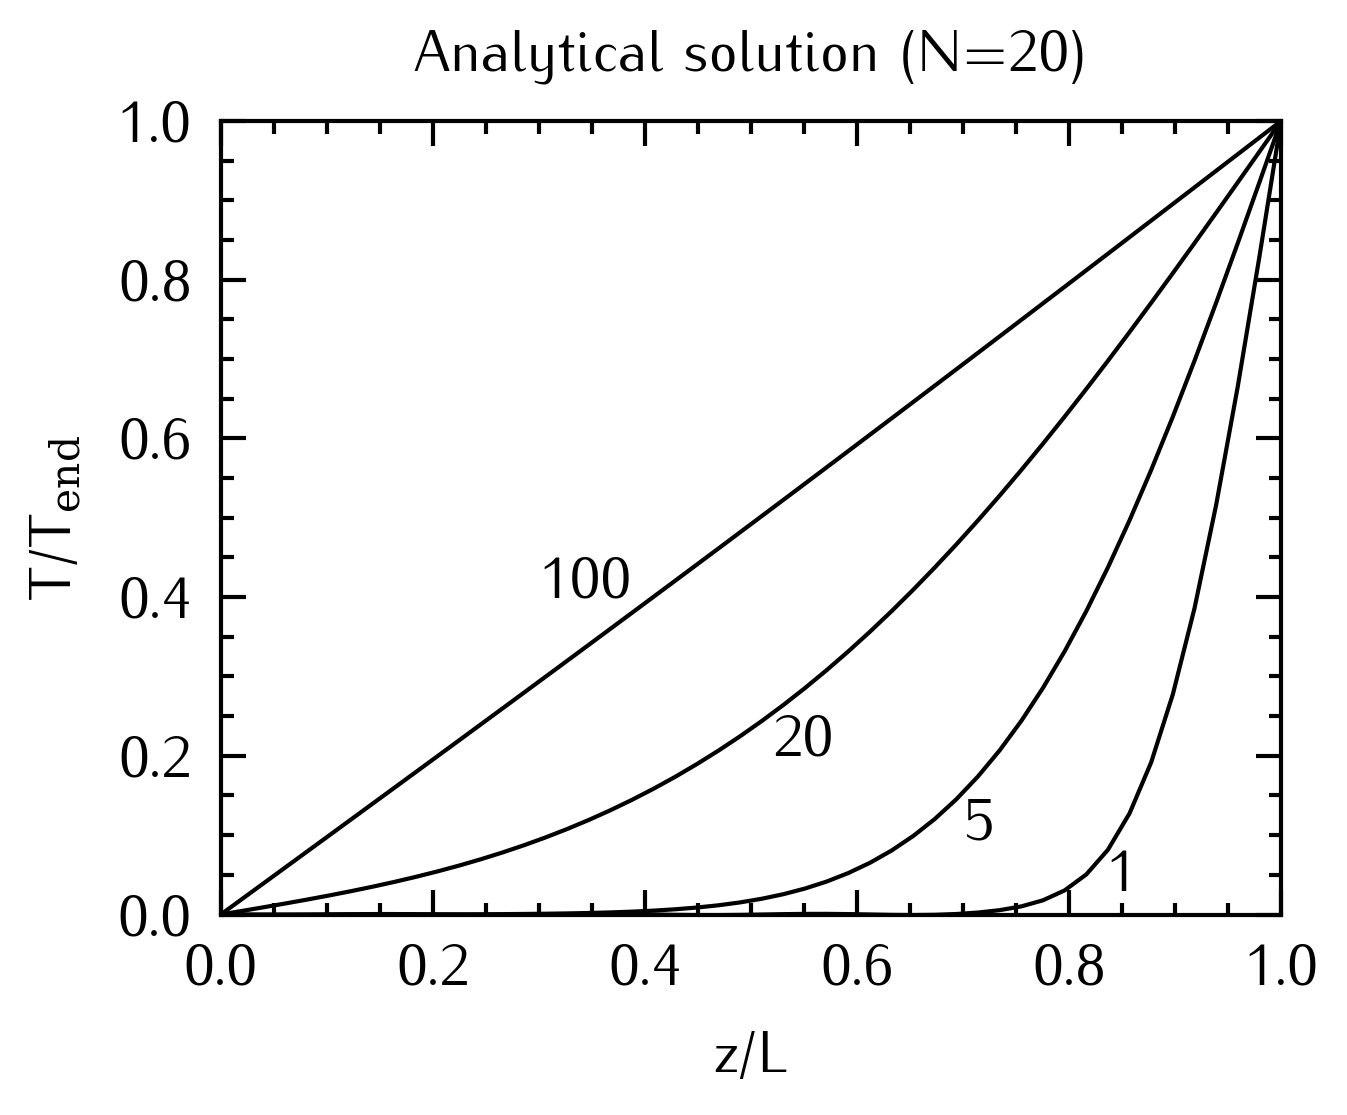
\includegraphics[width=60mm]{fig/step_analytical_sol.png}
\end{minipage}%
\begin{minipage}{.5\textwidth}
  \centering
  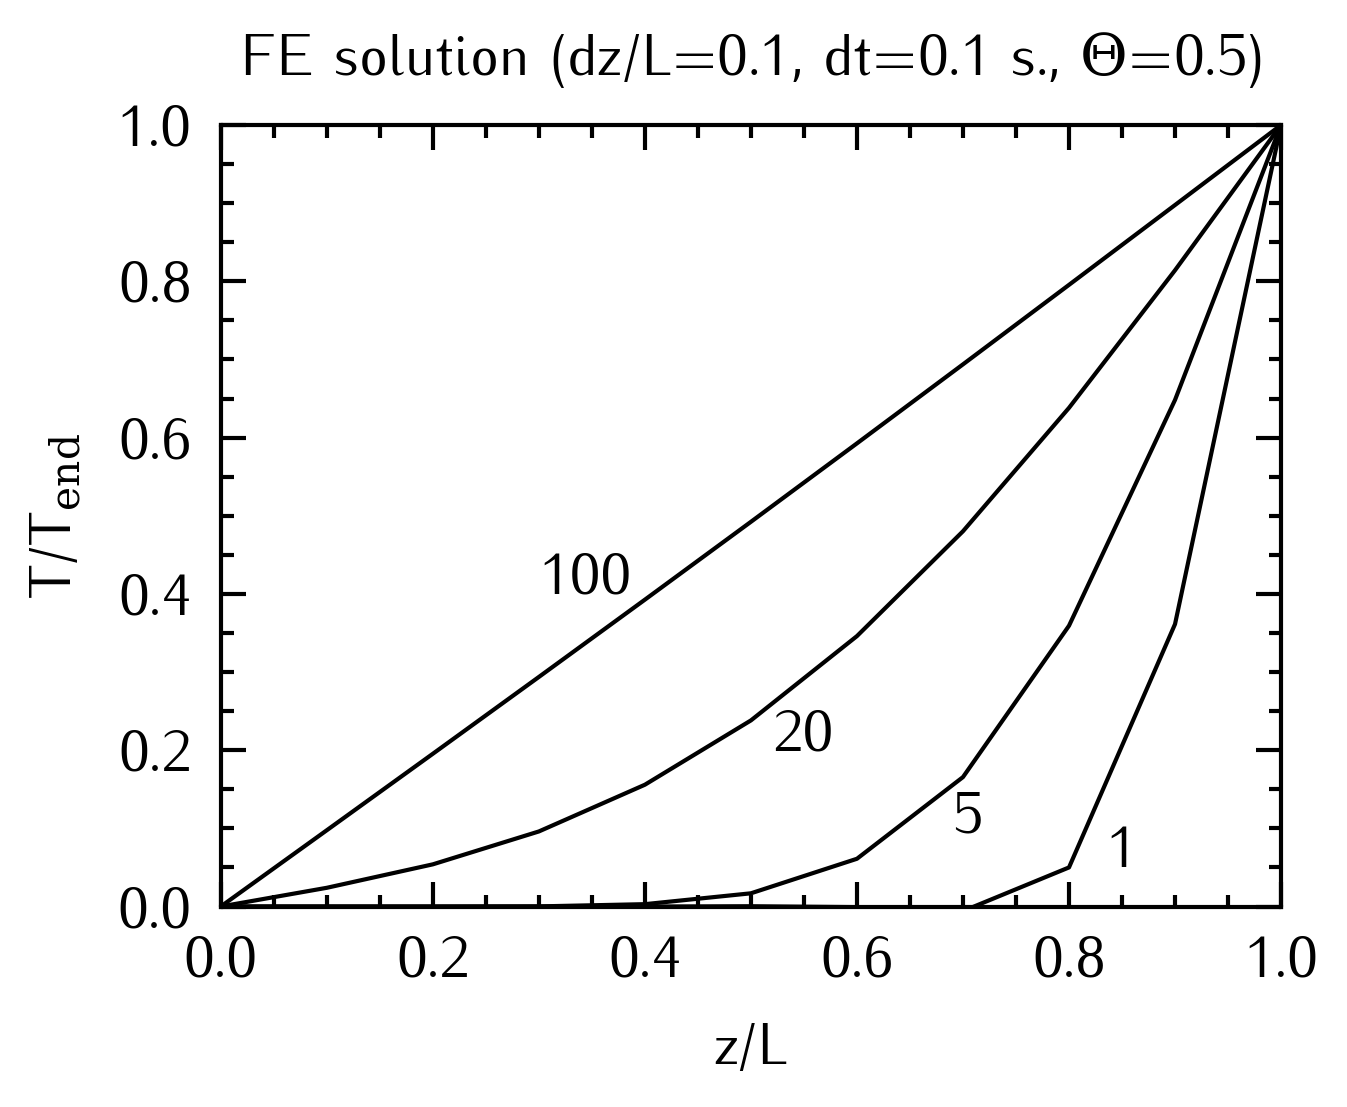
\includegraphics[width=60mm]{fig/step_FE_t0.5_dt0.1s.png}
\end{minipage}
\caption{Comparison of the analytical and FE solution at different times. The numbers in the graphs indicate the time in seconds.}
\label{fig:step_compare}
\end{figure}
\begin{table}[bt]
\centering
\caption{Domain properties.}
\label{tbl:prop}
\begin{tabular}{ll}
\textbf{Property}          & \textbf{Value} \\\hline
Domain length, $L$         & 0.01 m\\
Conductivity, $k$          & 0.72 W/m K\\
Density, $\rho$            & 1560 kg/m$^3$\\
Specific heat, $c_\text{p}$ & 1450 J/kg K\\\hline
\end{tabular}
\end{table}


\subsection{Constant heat flux at boundary of semi-infinite solid}
\label{sec:org57f413a}



\section{Use cases}
\label{sec:orga60ea4f}

\subsection{Press forming}
\label{sec:orgc42e2b2}

\subsection{Laser assisted fiber placement}
\label{sec:org44c2b41}
\end{document}